\chapter{Class Diagrams}

\section{First Cycle Design}
\label{sec:appendix1}
  \begin{figure}[!htb]
    \begin{center}
      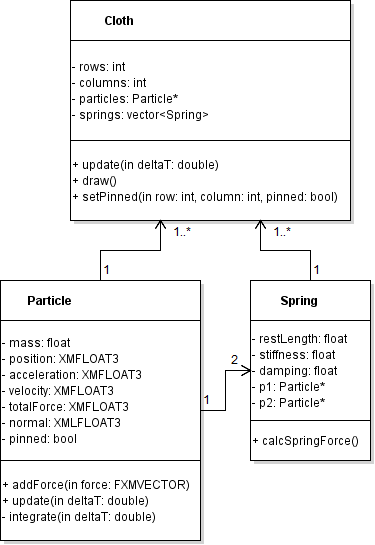
\includegraphics[scale=0.66]{Figures/cycle_1_initial_design}
    \end{center}
    \caption{Initial design for the first development cycle}
    \label{fig:phase1 initial}
  \end{figure}
  
  \begin{figure}
    \begin{center}
      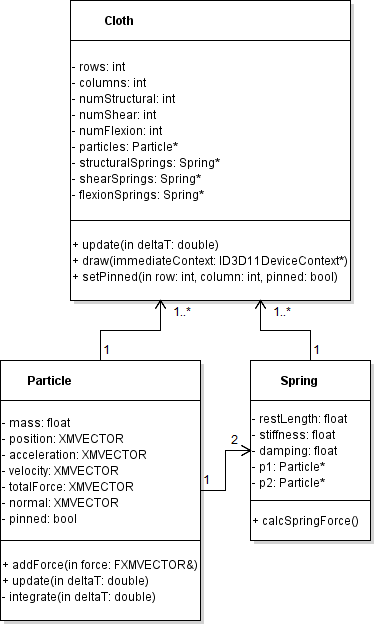
\includegraphics[scale=0.66]{Figures/cycle_1_final_design}
    \end{center}
    \caption{Final design for the first development cycle}
    \label{fig:phase1}
  \end{figure}
  
\begin{landscape}
\section{Second Cycle Design}
  \begin{figure}[!htb]
    \begin{center}
      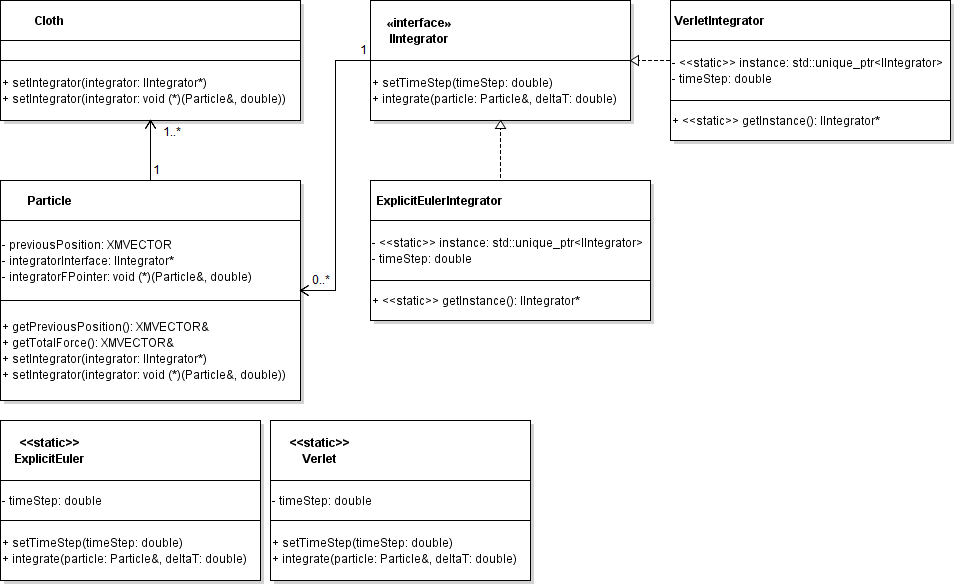
\includegraphics[scale=0.63]{Figures/cycle_2_initial_design}
    \end{center}
    \caption{Initial design for the second development cycle}
    \label{fig:phase2 initial}
  \end{figure}
  
  \begin{figure}
    \begin{center}
      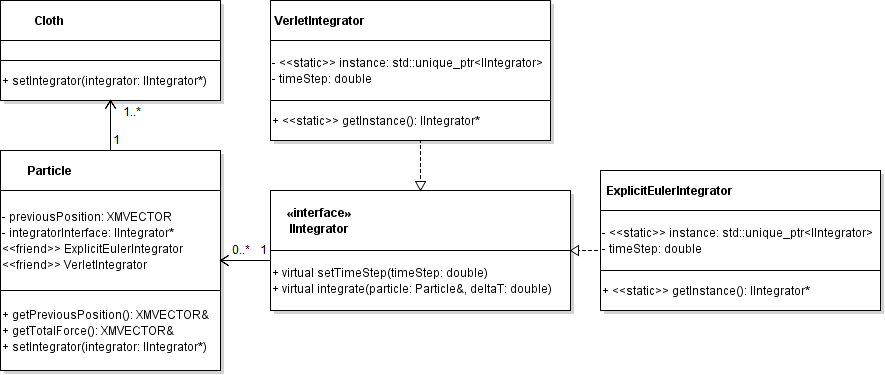
\includegraphics[scale=0.75]{Figures/cycle_2_final_design}
    \end{center}
    \caption{Final design for the second development cycle}
    \label{fig:phase2}
  \end{figure}
\end{landscape}

\section{Third Cycle Design}
  \begin{figure}[!htb]
    \begin{center}
      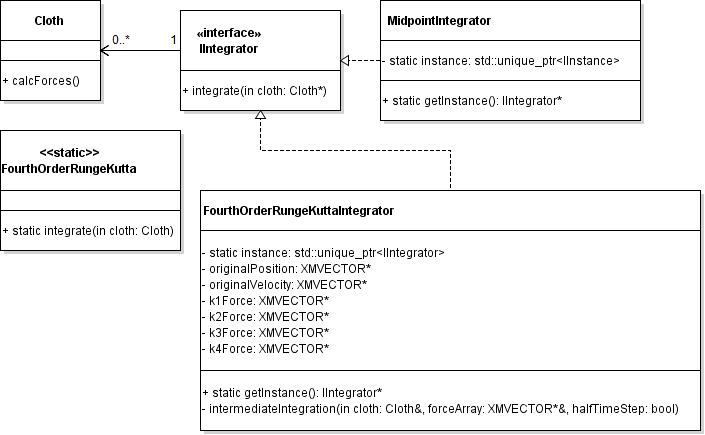
\includegraphics[scale=0.70]{Figures/cycle_3_initial_design}
    \end{center}
    \caption{Initial design for the third development cycle}
    \label{fig:phase3 initial}
  \end{figure}
  
  \begin{figure}
    \begin{center}
      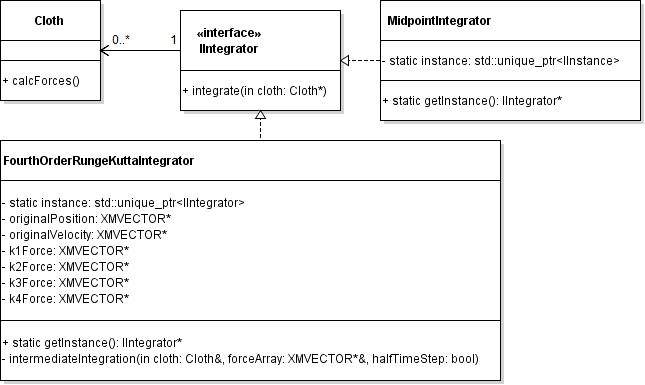
\includegraphics[scale=0.75]{Figures/cycle_3_final_design}
    \end{center}
    \caption{Final design for the third development cycle}
    \label{fig:phase3}
  \end{figure}

\begin{landscape}
\chapter{Profiling Results}

\section{First Cycle}
  \begin{figure}[!htb]
    \begin{center}
      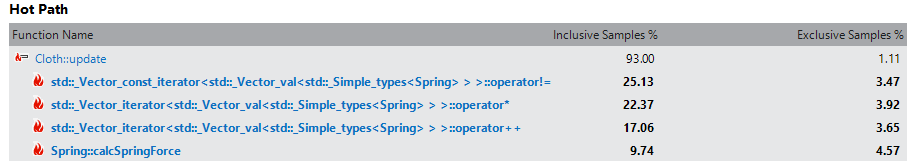
\includegraphics[scale=1.0]{Figures/vector_profiling_before}
    \end{center}
    \caption{Profiling results using an std::vector to store springs}
    \label{fig:profiling1}
  \end{figure}
  
    \begin{figure}
    \begin{center}
      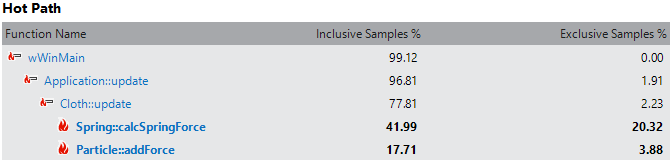
\includegraphics[scale=1.0]{Figures/vector_profiling_after}
    \end{center}
    \caption{Profiling results using dynamic arrays to store springs}
    \label{fig:profiling2}
  \end{figure}
  
    \begin{figure}[!htb]
    \begin{center}
      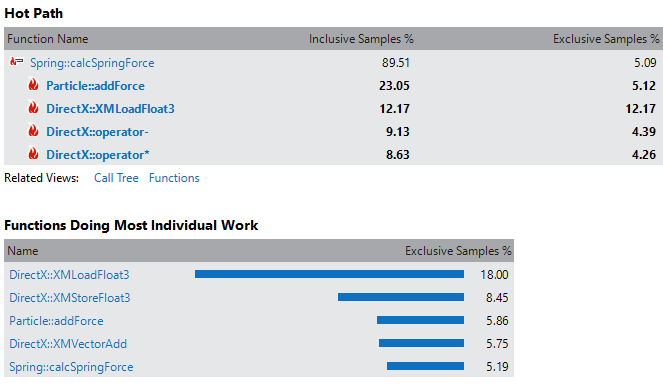
\includegraphics[scale=1.0]{Figures/calcspringforce_profiling_before}
    \end{center}
    \caption{Profiling results for unoptimised calcSpringForce}
    \label{fig:profiling3}
  \end{figure}
  
    \begin{figure}[!htb]
    \begin{center}
      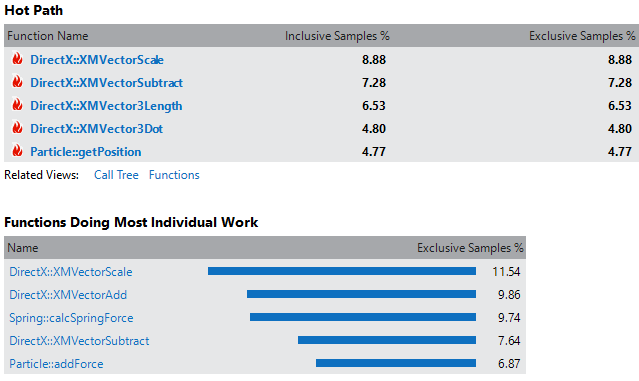
\includegraphics[scale=1.0]{Figures/calcspringforce_profiling_after}
    \end{center}
    \caption{Profiling results for optimised calcSpringForce}
    \label{fig:profiling4}
  \end{figure}
\end{landscape}